% --------------------------------------------------------------
% This is all preamble stuff that you don't have to worry about.
% Head down to where it says "Start here"
% --------------------------------------------------------------
 
\documentclass[12pt]{article}
 
\usepackage[margin=1in]{geometry} 
\usepackage{amsmath,amsthm,amssymb}
\usepackage{tikz}
\usetikzlibrary{arrows,shapes,trees} % loads some tikz extensions
 
\begin{document}
 
% --------------------------------------------------------------
%                         Start here
% --------------------------------------------------------------
 
\title{Homework 1}%replace X with the appropriate number
\author{Josh Klontz\\ %replace with your name
CSE 802} %if necessary, replace with your course title
 
\maketitle
\begin{enumerate}
\item
  \begin{enumerate}
  \item \textbf{Why would a packaging company be interested in automating this classification problem?} \\
    A packaging company would be interested in automatic vegetable classification in order to mechanically sort vegetables by type for boxing.
    There are at least three distinct advantages to having a machine sort the vegetables instead of a human.
    First, machine sorting may be faster and more cost effective than human sorting.
    Second, the machine may be able to handle the produce more delicately than a human thus reducing the chance of damaging it.
    Lastly, from a food borne disease aspect, reducing the number of people in the packaging plant decreases the chance of a sick worker infecting the produce.
  \item \textbf{What kind of sensors must be used? Show a schematic diagram of the sensor arrangement.} \\
    A camera must be used in order determine when there are vegetables to be sorted and to provide visual data as to what kind of vegetable it is.
    A scale might also provide helpful information. \\
    \begin{figure}[h]
    \centering
    \small
    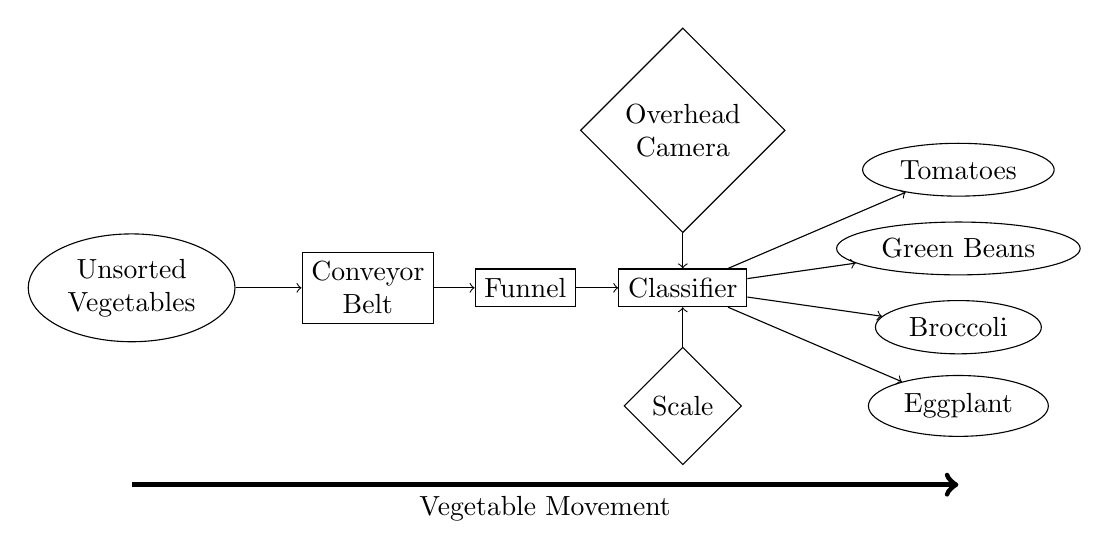
\begin{tikzpicture}
      \node[draw,ellipse,align=center] (a) at (0, 2.5) {Unsorted\\Vegetables};
      \node[draw,rectangle,align=center] (b) at (3,2.5) {Conveyor\\Belt};
      \node[draw,rectangle] (c) at (5,2.5) {Funnel};
      \node[draw,rectangle] (d) at (7,2.5) {Classifier};
      \node[draw,diamond,align=center] (e) at (7,4.5) {Overhead\\Camera};
      \node[draw,diamond] (f) at (7,1) {Scale};
      \node[draw,ellipse] (g) at (10.5,4) {Tomatoes};
      \node[draw,ellipse] (h) at (10.5,3) {Green Beans};
      \node[draw,ellipse] (i) at (10.5,2) {Broccoli};
      \node[draw,ellipse] (j) at (10.5,1) {Eggplant};
      \draw[->] (a) -- (b);
      \draw[->] (b) -- (c);
      \draw[->] (c) -- (d);
      \draw[->] (e) -- (d);
      \draw[->] (f) -- (d);
      \draw[->] (d) -- (g);
      \draw[->] (d) -- (h);
      \draw[->] (d) -- (i);
      \draw[->] (d) -- (j);
      \draw[->,line width=2pt] (0,0) -- (10.5,0) node[pos=.5,sloped,below] {Vegetable Movement};
    \end{tikzpicture}
    \caption{Sensor schematic diagram.}
    \end{figure}
  \item \textbf{What kind of preprocessing or segmentation can be done to make the resulting object representation (feature extraction) convenient for further processing?
    What features will be useful for separating these four classes?} \\
    The most important preprocessing step is to separate vegetables so that they do not overlap or touch.
    This ensures that when a vegetable appears in front of the camera its contour can be readily segmented from the background for color and shape analysis.
    It also facilitates directing each individual vegetable into its appropriate box after classification.
    Choosing a distinct background color like white, yellow, orange, or pink will help make automated segmentation for reliable.
    \par
    Hue is the most useful feature to separate the vegetables.
    It should readily identify tomatoes (red) from eggplants (purple) from green beans/broccoli (green).
    Table \ref{tbl:vegfeatures} shows three features that could be considered to separate green beans from broccoli.
    \begin{table}[h]
      \centering
      \begin{tabular}{l | c c}
        & \textbf{Green Beans} & \textbf{Broccoli} \\
        \hline
        \textbf{Weight} & Low & High \\
        \textbf{Area} & Low & High \\
        \textbf{Area/Perimeter} & Low & High \\
      \end{tabular}
      \caption{Features that distinguish green beans from broccoli.}
      \label{tbl:vegfeatures}
    \end{table}
  \item \textbf{What are the challenges involved in representing the vegetables, and how will the features you proposed help in overcoming these challenges?} \\
    The challenge in representing vegetables is finding features that are invariant to orientation, illumination, and size. $Hue$ and $Area/Perimeter$ are invariant to all three of these challenges. While $Weight$ and $Area$ are not invariant to vegetable size, the dramatic size difference between green beans and broccoli still allow them to be useful.
  \end{enumerate}
\end{enumerate}

 
% --------------------------------------------------------------
%     You don't have to mess with anything below this line.
% --------------------------------------------------------------
 
\end{document}